%%%%%%%%%%%%%%%%%%%%%%%%%%%%%%%%%%%%%%%%%%%%%%%%%%%%%%%%%%%%%%%%%%%%%%%%%%%%%%%%%%%%%%%%%%%
%% Ultimas modificacoes, 06/02/2012 - Alexandre Duarte 
%% Baseado no modelo latex de Isaac Maia (COPIN/UFCG)
%%
%% Para utilizar ese modelo sao necessarios os seguintes arquivos:
%%
%% ppgi.cls
%% ppgi.sty
%% mestre.sty
%%
%%
%% Mais detalhes sobre normas ABNT no latex, consultar http://abntex.codigolivre.org.br
%% Wiki interessante com dicas uteis sobre latex : http://www.tex-br.org
%%
%%
%% Para compilar esse arquivo, e' sempre importante fazer duas passagens com latex
%%%%
%%%%%%%%%%%%%%%%%%%%%%%%%%%%%%%%%%%%%%%%%%%%%%%%%%%%%%%%%%%%%%%%%%%%%%%%%%%%%%%%%%%%%%%%%%%

\documentclass[a4paper,titlepage]{ppgi}\usepackage[]{graphicx}\usepackage[]{color}
%% maxwidth is the original width if it is less than linewidth
%% otherwise use linewidth (to make sure the graphics do not exceed the margin)
\makeatletter
\def\maxwidth{ %
  \ifdim\Gin@nat@width>\linewidth
    \linewidth
  \else
    \Gin@nat@width
  \fi
}
\makeatother

\definecolor{fgcolor}{rgb}{0.345, 0.345, 0.345}
\newcommand{\hlnum}[1]{\textcolor[rgb]{0.686,0.059,0.569}{#1}}%
\newcommand{\hlstr}[1]{\textcolor[rgb]{0.192,0.494,0.8}{#1}}%
\newcommand{\hlcom}[1]{\textcolor[rgb]{0.678,0.584,0.686}{\textit{#1}}}%
\newcommand{\hlopt}[1]{\textcolor[rgb]{0,0,0}{#1}}%
\newcommand{\hlstd}[1]{\textcolor[rgb]{0.345,0.345,0.345}{#1}}%
\newcommand{\hlkwa}[1]{\textcolor[rgb]{0.161,0.373,0.58}{\textbf{#1}}}%
\newcommand{\hlkwb}[1]{\textcolor[rgb]{0.69,0.353,0.396}{#1}}%
\newcommand{\hlkwc}[1]{\textcolor[rgb]{0.333,0.667,0.333}{#1}}%
\newcommand{\hlkwd}[1]{\textcolor[rgb]{0.737,0.353,0.396}{\textbf{#1}}}%

\usepackage{framed}
\makeatletter
\newenvironment{kframe}{%
 \def\at@end@of@kframe{}%
 \ifinner\ifhmode%
  \def\at@end@of@kframe{\end{minipage}}%
  \begin{minipage}{\columnwidth}%
 \fi\fi%
 \def\FrameCommand##1{\hskip\@totalleftmargin \hskip-\fboxsep
 \colorbox{shadecolor}{##1}\hskip-\fboxsep
     % There is no \\@totalrightmargin, so:
     \hskip-\linewidth \hskip-\@totalleftmargin \hskip\columnwidth}%
 \MakeFramed {\advance\hsize-\width
   \@totalleftmargin\z@ \linewidth\hsize
   \@setminipage}}%
 {\par\unskip\endMakeFramed%
 \at@end@of@kframe}
\makeatother

\definecolor{shadecolor}{rgb}{.97, .97, .97}
\definecolor{messagecolor}{rgb}{0, 0, 0}
\definecolor{warningcolor}{rgb}{1, 0, 1}
\definecolor{errorcolor}{rgb}{1, 0, 0}
\newenvironment{knitrout}{}{} % an empty environment to be redefined in TeX

\usepackage{amsmath}
\usepackage{alltt}
\usepackage[portuguese,ruled,linesnumbered]{algorithm2e}
\usepackage[english,portuges]{babel}
\usepackage{ppgi,mestre,epsfig}
\usepackage{times}
\usepackage[final]{pdfpages}
\usepackage{hyperref}
\hypersetup{
    bookmarks=true,   
    pdftitle={Monitor legislativo},
    pdfauthor={Vitor Márcio Paiva de Sousa Baptista}, 
    pdfsubject={Modelo de Documento Científico},
    pdfkeywords={Dissertação, Mestrado, PPGI, UFPB, modelo}, 
    colorlinks=true,
    linkcolor=black,
    citecolor=black,
    filecolor=black,
    urlcolor=black
 }

% Corrige bug no algorithm2e que usa termos em espanhol ao invés de português
\SetKwFor{Para}{para}{fa\c{c}a}{fim para}
\SetKwFor{ParaPar}{para}{fa\c{c}a em paralelo}{fim para}
\SetKwFor{ParaCada}{para cada}{fa\c{c}a}{fim para cada}
\SetKwFor{ParaTodo}{para todo}{fa\c{c}a}{fim para todo}

%-------------------------- Para usar acentuacaoo em sistemas ISO8859-1 ------------------------------------
% Se estiver usando o Microsoft Windows ou linux com essa codificacao, descomente essas linhas abaixo
% e comente as linhas referentes ao UTF8
%\usepackage[applemac]{inputenc} % Usar acentuacao em sistemas ISO8859-1, comentar a linha com  \usepackage[utf8x {inputenc}
%-----------------------------------------------------------------------------------------------------

%-------------------------- Para usar acentuacao em sistemas UTF8 ------------------------------------
% Para a maior parte das distribuicoes linux, usar essa opcao
\usepackage{ucs}
\usepackage[utf8x]{inputenc}
\usepackage[T1]{fontenc}
%-----------------------------------------------------------------------------------------------------
\usepackage{float}      
\usepackage{fancyvrb}
\usepackage{fancyheadings}
\usepackage{tikz} % Permite usar math mode dentro dos gráficos do knitr
\usepackage{graphicx}
\graphicspath{{figure/}}
\setkeys{Gin}{width=0.5\textwidth}
\usepackage{longtable} %tabelas longas, para tabelas que ultrapassam uma pagina
\usepackage{pdflscape} % landscape figures
\usepackage{glossaries} % Gerar glossário
\usepackage[skip=0pt]{caption} % Diminui distância entre imagens/tabelas e seus captions
\usepackage{subcaption}
\newcommand{\subfloat}[2][need a sub-caption]{\subcaptionbox{#1}{#2}}

\makeglossaries
\newacronym{IR}{IR}{Índice de Rice}
\newacronym{PT}{PT}{Partido dos Trabalhadores}
\newacronym{PSOL}{PSOL}{Partido Socialismo e Liberdade}
\newacronym{API}{API}{\emph{Application Programming Interface}}
\newacronym{XML}{XML}{\emph{eXtensible Markup Language}}
\newacronym{CSV}{CSV}{\emph{Comma Separated Values}}
\newacronym{JSON}{JSON}{\emph{JavaScript Object Notation}}
\newacronym{CEBRAP}{CEBRAP}{Centro Brasileiro de An\'alise e Pesquisa}

%\input{psfig.sty}
% ----------------- Para inserir codigo fonte de linguagens de programacao no documento -------------
\usepackage{listings}
\lstset{numbers=left,
stepnumber=1,
firstnumber=1,
numberstyle=\scriptsize,
extendedchars=true,
breaklines=true,
frame=tb,
basicstyle=\scriptsize,
stringstyle=\ttfamily,
showstringspaces=false
}
\renewcommand{\lstlistingname}{C\'odigo Fonte}
\renewcommand{\lstlistlistingname}{Lista de C\'odigos Fonte}

% ---------------------------------------------------------------------------------------------------

\selectlanguage{portuges}
\sloppy

\setcounter{secnumdepth}{4}
\setcounter{tocdepth}{4}
\usepackage{abnt-alf}

% Centraliza todos os floats
\makeatletter
\g@addto@macro\@floatboxreset\centering
\makeatother
\IfFileExists{upquote.sty}{\usepackage{upquote}}{}
\begin{document}


%%%%%%%%%%%%%%%%%%%%%%%%%%%%%%%%%%%%%%%%%%%%%%%%%%%%%%%%%%%%%%%%%%%%%%%%%%%%%%%%
\Titulo{Um modelo para a previsão da entrada ou saída\\da coalizão pelos deputados federais}
\Autor{Vitor Márcio Paiva de Sousa Baptista}
\Data{06 de Março de 2012}
\Area{Ciência da Computação}
\Pesquisa{Computação Distribuída | Sinais, Sistemas Digitais e Gráficos}
\Orientadores{Alexandre Nóbrega Duarte\\ (Orientador)}

\newpage
\cleardoublepage
\PaginadeRosto

\newpage
\cleardoublepage

%%%%%%%%%%%%%%%%%%%%%%%%%%%%%%%%%%%%%%%%%%%%%%%%%%%%%%%%%%%%%%%%%%%%%%%%%%%%%%%%
\begin{resumo} 
No Brasil, existem ferramentas para o acompanhamento do comportamento dos
parlamentares em votações nominais, tais como o Basômetro do jornal O Estado de
São Paulo e o Radar Parlamentar. Essas ferramentas são usadas para análises
tanto por jornalistas quanto por cientistas políticos.

Apesar de serem ótimas ferramentas de análise, sua utilidade para monitoramento
é limitada por exigir um acompanhamento manual, o que se torna muito trabalhoso
quando consideramos o volume de dados. Somente na Câmara dos Deputados, 513
parlamentares participam em média de mais de 400 votações nominais por
legislatura. É possível diminuir a quantidade de dados analisando os partidos
como um todo, mas em contrapartida perdemos a capacidade de detectar
movimentações de indivíduos ou grupos intrapartidários como as bancadas.

% FIXME: Estava falando de análise de comportamento em geral, e aqui já pulei
% para mudanças de posicionamento. Falta algo para ligar os dois.

Para diminuir esse problema, desenvolvi neste trabalho um modelo estatístico
que detecta quando um parlamentar muda de posicionamento, entrando ou saindo da
coalizão governamental, através de estimativas de pontos ideais usando o
W-NOMINATE. Ele pode ser usado individualmente ou integrado a ferramentas como
o Basômetro, oferecendo um filtro para os pesquisadores encontrarem os
parlamentares que mudaram mais significativamente de comportamento.

O universo de estudo é composto pelos parlamentares da Câmara dos Deputados no
período da 50\textordfeminine{} até a 54\textordfeminine{} legislaturas,
iniciando no primeiro mandato de Fernando Henrique Cardoso em 1995 até o final
do primeiro mandato de Dilma Rousseff em 2015.
\\
\\
\textbf{Palavras-chave:} Análise legislativa, Ciência política, Ciência de
dados, Modelos preditivos, Aprendizagem de máquina.

% FIXME: Faltou falar um pouco dos resultados.

\end{resumo}
%\newpage
%\cleardoublepage

%%%%%%%%%%%%%%%%%%%%%%%%%%%%%%%%%%%%%%%%%%%%%%%%%%%%%%%%%%%%%%%%%%%%%%%%%%%%%%%%
\begin{summary}
In Brazil, there are tools for monitoring the behaviour of legislators in
rollcalls, such as O Estado de São Paulo's Basômetro and Radar Parlamentar.
These tools are used both by journalists and political scientists for analysis.

Although they are great analysis tools, their usefulness for monitoring is
limited because they require a manual follow-up, which makes it a lot of work
when we consider the volume of data. Only in the Chamber of Deputies, 513
legislators participate on average over than 400 rollcalls by legislature. It
is possible to decrease the amount of data analyzing the parties as a whole,
but in contrast we lose the ability to detect individuals' drives or
intra-party groups such as factions.

In order to mitigate this problem, I developed a statistical model that detects
when a legislator changes his or her position, joining or leaving the
governmental coalition, through ideal points estimates using the W-NOMINATE. It
can be used individually or integrated to tools such as Basômetro, providing a
filter for researchers find the deputies who changed their behaviour most
significantly.

The universe of study is composed of legislators from the Chamber of Deputies
from the 50th to the 54th legislatures, starting in the first term of Fernando
Henrique Cardoso in 1995 until the end of the first term of Dilma Rousseff in
2015.

\textbf{Keywords:} Legislative Analysis, Political Science, Data Science,
Predictive Models, Machine Learning.

\end{summary}

%\newpage
%\cleardoublepage

%%%%%%%%%%%%%%%%%%%%%%%%%%%%%%%%%%%%%%%%%%%%%%%%%%%%%%%%%%%%%%%%%%%%%%%%%%%%%%%%
% TMP: Agradecimentos
\begin{agradecimentos}
Devo todas as conquistas de minha vida a minha família. Foi o seu
trabalho, amor e dedicação que me ensinaram e me permitiram fazer o que fiz. Se
todos chegamos aonde estamos por nos apoiarmos nos ombros de gigantes, foram
eles e elas os primeiros gigantes nos quais me apoiei.

Agradeço em especial a minha esposa, melhor amiga e coorientadora não-oficial
Samara. Sem sua ajuda, esse trabalho não seria possível e minha vida seria
muito mais solitária.

Agradeço também ao meu orientador, Alexandre. Só o conheci ao me inscrever no
mestrado, mas ao longo desses anos tive certeza que não poderia ter tido mais
sorte nessa escolha. Por sua orientação técnica, mas principalmente pelo seu
interesse indiscutível nessa área de pesquisa. Em outra situação, acredito que
ele mesmo teria escrito esse trabalho, o que é prova inegável da nossa
sintonia.

Agradeço as professoras Andréa Freitas e Thaís Gaudêncio, que aceitaram
participar da minha banca, emprestando seu tempo e conhecimento para a melhoria
deste trabalho.

Agradeço aos pesquisadores e funcionários do \gls{CEBRAP}, cuja contribuição à
área da Ciência Política é incalculável, no Brasil e no mundo. Em especial,
gostaria de agradecer a Andréa Freitas, ao Samuel Moura e ao Maurício Izumi, que 
me ajudaram muito a validar as ideias que discuti nesse trabalho, e ao Paulo
Hubert, que me auxiliou a acessar o banco de dados legislativos do
\gls{CEBRAP}, do qual extraí a lista de coalizões usada. Além, é claro, a
Argelina Figueiredo e o Fernando Limongi, cuja pesquisa foi um divisor de águas
no pensamento da Ciência Política brasileira.

Ao longo do tempo, o contato com pessoas interessadas na intersecção entre
computação, política e jornalismo foi abrindo meus olhos para essa nova área
que acho extremamente interessante. Isso foi possibilitado, principalmente,
pela criação do grupo Transparência Hacker por, entre tantos outros, Pedro
Markun e Daniela Silva. Através desse grupo, conheci pessoas fenomenais como os
jornalistas Daniel Bramatti, José Roberto de Toledo e Amanda Rossi que, junto
com o Diego Rabatone, formavam o Estadão Dados, onde tive o prazer de trabalhar
por uma semana durante o segundo turno das eleições de 2012.

Agradeço aos amigos criados durante a organização do Encontro de Software Livre
da Paraíba (ENSOL), em especial a Rodrigo Vieira e Anahuac de Paula Gil, os
principais responsáveis no meu amadurecimento com relação a software e cultura
livres.

Trabalhando na ThoughtWorks em Porto Alegre, fiz diversos amigos. Em especial,
Leonardo Tartari e Thiago Bueno, companheiros de vários hackathons, foram quem
despertaram em mim o interesse pela visualização de dados, que foi uma das
razões que me fizeram entrar na Open Knowledge Foundation (OKF).

A OKF é uma ONG inglesa que trabalha com dados abertos. Durante os anos que
trabalhei nela, tive oportunidade de conhecer diversas pessoas que me ajudaram
a me aprofundar nessa área, em especial o time de desenvolvimento do CKAN e os
fundadores da Open Knowledge Foundation Brasil.

Por último, mas de forma alguma menos importante, agradeço aos amigos brutais,
os irmãos e irmãs que encontrei durante a vida. Em especial ao Pedro Guimarães
que, além de amigo e parceiro em diversos projetos, se tornou meu cunhado.

À todas essas pessoas e muitas outras, dedico esse trabalho.

\end{agradecimentos}

\clearpage

%%%%%%%%%%%%%%%%%%%%%%%%%%%%%%%%%%%%%%%%%%%%%%%%%%%%%%%%%%%%%%%%%%%%%%%%%%%%%%%%
%% Definicao do cabecalho: secao do lado esquerdo e numero da pagina do lado direito
\pagestyle{fancy}
\addtolength{\headwidth}{\marginparsep}\addtolength{\headwidth}{\marginparwidth}\headwidth = \textwidth
\renewcommand{\chaptermark}[1]{\markboth{#1}{}}
\renewcommand{\sectionmark}[1]{\markright{\thesection\ #1}}\lhead[\fancyplain{}{\bfseries\thepage}]%
	     {\fancyplain{}{\emph{\rightmark}}}\rhead[\fancyplain{}{\bfseries\leftmark}]%
             {\fancyplain{}{\bfseries\thepage}}\cfoot{}

%%%%%%%%%%%%%%%%%%%%%%%%%%%%%%%%%%%%%%%%%%%%%%%%%%%%%%%%%%%%%%%%%%%%%%%%%%%%%%%%

\Sumario
\ListadeSiglas
\listoffigures
\listoftables
\lstlistoflistings %lista de codigos fonte - Para inserir a listagem de
% codigos fonte

\newpage
\cleardoublepage
\Introducao


%%%%%%%%%%%%%%%%%%%%%%%%%%%%%%%%%%%%%%%%%%%%%%%%%%%%%%%%%%%%%%%%%%%%%%%%%%%%%%%%
%
% Hifenizacao - Colocar lista de palavras que nao devem ser separadas e que 
% nao estao no dicionario portuges.
% As palavras do dicionario portuges ja sao separadas corretamente pelo lateX
%
\hyphenation{ gLite OurGrid GridDoctor }

%%%%%%%%%%%%%%%%%%%%%%%%%%%%%%%%%%%%%%%%%%%%%%%%%%%%%%%%%%%%%%%%%%%%%%%%%%%%%%%%
%% A partir daqui coloque seus capitulos. Sugere-se que eles sejam inseridos com o comando \input
%% Da seguinte maneira:
%% 



\chapter{Introdução} \label{intro}

Neste capítulo, serão descritos o que motivou o desenvolvimento deste trabalho
(Seção \ref{sec:motivacao}), juntamente com a definição do problema e objetivos
da pesquisa, a metodologia seguida, publicações relacionadas e, por fim, será
resumida a estrutura do restante da dissertação.

\section{Motivação}\label{sec:motivacao}

O acompanhamento das atividades dos legisladores é extremamente importante,
pois são eles que alteram as leis do Brasil. Isso afeta todos que têm alguma
relação com o país, estando ou não em solo brasileiro. As grandes empresas,
com recurso para investir, reconhecem a importância de acompanhar de perto a
atividade legislativa, seja passiva ou ativamente através de \emph{lobbying}.
Infelizmente, com exceção das leis que são divulgadas na mídia, como aumentos
do salário mínimo ou, recentemente, a redução da maioridade penal, a maioria
dos cidadãos não se interessa por essa área, seja por falta de tempo,
conhecimento ou simplesmente falta de interesse.

Jornalistas políticos exercem um papel fundamental nesse sentido, traduzindo os
termos técnicos e jurídicos usados pelos parlamentares em uma forma que possa
ser mais facilmente compreendida pelo cidadão comum. Entretanto, como essa
análise demanda bastante tempo, ela acaba se restringindo aos temas mais
polêmicos, que atingem um maior número de pessoas. Esses temas são muito
importantes, mas não suficientes: se eu trabalho numa ONG de preservação do
meio ambiente, por exemplo, meu maior interesse é em projetos de lei que versem
sobre essa área.

Percebendo essa necessidade, empresas como o \gls{ELLO} no Brasil e a
FiscalNote nos Estados Unidos, criaram ferramentas que facilitam esse
monitoramento personalizado. Seus produtos permitem que o usuário defina suas
áreas de interesse (por exemplo, meio ambiente ou mobilidade urbana),
recebendo resumos periódicos do que as afeta, inclusive com previsões da
probabilidade de aprovação dos projetos de lei relacionados a elas. Apesar
disso, por serem ferramentas pagas, seu uso ainda é restrito.

% Explica importância do monitoramento do comportamento dos legisladores
Um dos fatores mais importantes no comportamento dos parlamentares é o conflito
governo/oposição \cite{Leoni2002,Desposato2005b,Freitas2012,Izumi2013}. Diante
disso, quando um parlamentar muda de lado, seja migrando de partido ou quando
seu próprio partido se une (ou deixa) à coalizão governamental, é de se esperar
que seu comportamento também mude. Como, no geral, os partidos são capazes de
disciplinar seus filiados a votarem de certa forma, essa mudança de forças pode
definir a aprovação ou não de um projeto de lei. Assim, é essencial monitorar
essas mudanças para entender as chances que um projeto tem de ser aprovado.

Entretanto, o grande volume de dados gera um desafio. Considerando somente o
nível federal, 513 deputados federais e 81 senadores participam de centenas de
votações em cada legislatura, tornando difícil o entendimento dos seus padrões
de votação. Algumas ferramentas, como o Basômetro e o Radar Parlamentar, foram
criadas para tentar diminuir esse problema \cite{Estadao2012,Trento2013}.

Elas são ferramentas gratuitas que permitem o acompanhamento da taxa de
governismo (no caso do Basômetro) ou das posições relativas dos parlamentares
(no caso do Radar Parlamentar), auxiliando o cidadão comum a se aproximar do
processo legislativo \cite{Dantas2014}. Entretanto, mesmo facilitando bastante,
não é fácil analisar um gráfico com 513 pontos (no caso da Câmara) e visualizar
o que está mudando ou não. Para diminuir esse desafio, as análises acabam sendo
feitas baseadas no comportamento agregado dos partidos, e não dos parlamentares
individualmente.

Os partidos são capazes de influenciar o comportamento dos seus parlamentares,
mantendo taxas de disciplina, em sua maioria, acima de 75\%
\cite{Figueiredo2001,Cheibub2009,Zucco2009}. Assim, a análise a nível de partido
é uma forma importantíssima de entender o comportamento parlamentar. Apesar
disso, algumas informações são perdidas ao fazer essa agregação. Para dar um
exemplo concreto, o \gls{PT} é, historicamente, um dos partidos brasileiros mais
disciplinados. Em 2003, o primeiro ano do primeiro governo Lula, o \gls{PT} manteve uma
disciplina altíssima (98,36 \% na Câmara). Apesar disso, três deputados e uma
senadora constantemente votavam contrários a indicação do partido, o que acabou
resultando na sua expulsão no final do mesmo ano \cite{Breve2013}.

Esses parlamentares são os deputados Babá, Luciana Genro e João Fontes e a
senadora Heloísa Helena. Após serem expulsos, fundaram um novo partido: o
\gls{PSOL}. Essa movimentação passaria desapercebida ao analisar o \gls{PT}
como um todo, já que só 4 dos quase 100 deputados e senadores do partido
tiveram esse comportamento.

O objetivo deste trabalho é o desenvolvimento de um modelo estatístico que
determine a chance de um parlamentar ter mudado de posicionamento com base no
seu padrão de voto. Esse modelo foi treinado com os dados da
50\textordfeminine{} até a 54\textordfeminine{} legislaturas, compreendendo o
período de 20 anos de 1995, no início do primeiro governo de Fernando Henrique
Cardoso, até o início de 2015, no início do segundo governo de Dilma Rousseff.

Com isso, espero criar uma ferramenta para que os cidadãos, jornalistas e
cientistas políticos consigam filtrar e ordenar os parlamentares pela
intensidade da sua mudança de comportamento. Dessa forma, eles otimizariam o
uso do seu tempo, focando em quem está mudando. Esse modelo poderá ser usado
separadamente, ou integrado em ferramentas já existentes, como o Basômetro ou o
Radar Parlamentar, visando aumentar sua utilidade como ferramentas de
monitoramento legislativo.

Essa ferramenta poderá ser útil também para os próprios parlamentares,
especialmente os líderes, permitindo que monitorem se seus liderados estão
mudando de lado.

Como preditores, o modelo usa os pontos ideais dos parlamentares, estimados
pelo algoritmo W-NOMINATE \cite{Poole1985,Poole2005}. Além desses pontos,
também replicamos parte da pesquisa de \citeonline{Freitas2008}, que analisa os
aspectos temporais das migrações partidárias no Brasil, focando nas mudanças de
posicionamento, sejam a partir da migração para partidos de posicionamento
oposto (indo do governo para oposição ou vice-versa), ou na entrada ou saída do
próprio partido na coalizão governamental.

Uma das principais contribuições deste trabalho é democratizar o acesso a
técnicas antes só disponíveis em sistemas pagos de empresas como o \gls{ELLO}
e a FiscalNote.

\section{Problema de pesquisa}
\label{cap:introducao:problemas-de-pesquisa}

Os partidos e as coalizões governamentais são capazes de influenciar o
comportamento dos parlamentares \cite{Figueiredo2001,Santos2003}. Partindo
disso, \citeonline{Izumi2013} mostrou que o comportamento dos senadores muda ao
entrar ou sair da coalizão, mas não sabemos se ele muda antes ou depois da
oficialização dessa mudança. A pergunta a que buscamos responder neste trabalho
é:

\emph{É possível detectar a mudança de posicionamento de um deputado federal,
com ele entrando ou saindo da coalizão governamental, a partir de uma mudança
no seu padrão de votação?}

A premissa básica deste trabalho é que, além de ser possível detectar mudanças
de posicionamento, essa detecção ocorra antes da oficialização da mudança. Em
outras palavras, que o modelo seja capaz de detectar uma mudança de
posicionamento antes que ela seja do conhecimento público. Para isto,
precisaremos também responder à pergunta:

\emph{Os deputados federais mudam seu padrão de votação antes de mudarem de
posicionamento?}

Alguns autores mostraram que os parlamentares mudam de comportamento ao mudarem
de posicionamento (ver Capítulo \ref{cap:trabalhos-relacionados}). Apesar
disso, não foram encontrados trabalhos que discorram sobre se tal mudança de
comportamento ocorre antes ou depois da efetiva mudança de posicionamento.
Assim, responder a essa pergunta é uma outra contribuição deste trabalho.

\section{Objetivos}

O objetivo geral desta dissertação é o desenvolvimento e validação de um modelo
capaz de determinar a chance de um deputado federal ter mudado de
posicionamento em um determinado período.

Para alcançar esse objetivo geral, foram definidos os seguintes objetivos
específicos:

\begin{itemize}
  \item Determinar um conjunto de características a partir das quais seja
    possível determinar a chance de um parlamentar mudar de posicionamento;
  \item Descobrir se os parlamentares mudam de comportamento antes de mudarem
    de posicionamento;
  \item Analisar diversos modelos estatísticos, buscando qual tem melhor
    performance na detecção da mudança de posicionamento dos deputados
    federais brasileiros.
\end{itemize}

\section{Metodologia}

Para o desenvolvimento desta pesquisa, foram seguidos os seguintes passos:

\begin{enumerate}
  \item Levantamento bibliográfico sobre análise do comportamento parlamentar,
    análise da mudança do comportamento parlamentar, e métodos de aprendizado
    de máquina usados no âmbito da Ciência Política;
  \item Extração dos dados de votos e votações a partir da página da Câmara dos
    Deputados, e da listagem de coalizões a partir do banco de dados
    legislativo do \gls{CEBRAP};
  \item Definição da forma para representação desses dados, usando a teoria
    espacial do voto;
  \item Análise dos padrões gerais e temporais dos pontos ideais estimados;
  \item Definição de variáveis independentes capazes de serem usadas para
    diferenciar parlamentares que mudaram de posicionamento dos que não
    mudaram;
  \item Análise de diversos modelos preditivos buscando o que obtêm a melhor
    performance nesses dados;
  \item Validação do modelo final baseado na análise feita na etapa anterior.
\end{enumerate}

\section{Publicações Relacionadas}

Resultados iniciais desta pesquisa foram publicados no artigo ``Uma ferramenta
para analisar mudanças na coesão entre parlamentares em votações nominais'',
apresentado no III Brazilian Workshop on Social Network Analysis and Mining
(BRASNAM), ocorrido em 2014 \cite{Baptista2014}.

\section{Estrutura da Dissertação}

Esta dissertação é dividida em cinco capítulos, incluindo este introdutório,
que apresentou a motivação, problema de pesquisa e objetivos deste trabalho.

No Capítulo \ref{cap:fundamentacao}, \nameref{cap:fundamentacao}, serão
brevemente apresentados os conceitos básicos necessários para entendimento do
restante do trabalho. Na Seção \ref{cap:fundamentacao:ciencia-de-dados}, falarei
sobre a Ciência de Dados, com foco no desenvolvimento de modelos preditivos
para predição de variáveis categóricas e sua validação através de matrizes de
confusão e ferramentas como a curva \gls{ROC}.

Na Seção \ref{cap:fundamentacao:teoria-espacial-do-voto}, apresentarei técnicas
baseadas na teoria espacial do voto, que permitem colocar um conjunto de
parlamentares em um plano cartesiano, com suas posições definidas a partir de
seus votos em um conjunto de votações. Existem diversas técnicas para definir
essas posições, mas neste trabalho focarei no W-NOMINATE, uma das mais usadas.

Na Seção \ref{cap:fundamentacao:comparando-pontos-ideais-no-tempo}, será
apresentado o problema em comparar pontos ideais ao longo do tempo, descrevendo
técnicas que usam ``pontes'' para diferenciar mudanças causadas por diferenças
na agenda legislativa dos períodos das causadas pela mudança de comportamento
do parlamentar.

No Capítulo \ref{cap:trabalhos-relacionados},
\nameref{cap:trabalhos-relacionados}, serão resumidos alguns trabalhos,
encontrados durante a revisão bibliográfica feita nesta pesquisa, que versam
sobre a análise do comportamento parlamentar, a mudança de comportamento e o
uso de técnicas de aprendizagem de máquina na Ciência Política.

Explicadas, até este momento, as ferramentas usadas no trabalho e a literatura
da área, no Capítulo \ref{cap:desenvolvimento}, \nameref{cap:desenvolvimento},
será descrito o processo de criação do modelo, partindo da definição do
universo de estudo, coleta e preparação dos dados, gerando estimativas dos
pontos ideais dos parlamentares, passando pela análise das características
gerais e temporais dos dados para, finalmente, descrever o desenvolvimento e
validação do modelo na Seção \ref{cap:desenvolvimento:modelagem},
\nameref{cap:desenvolvimento:modelagem}.

Por fim, o Capítulo \ref{cap:conclusao}, \nameref{cap:conclusao}, apresenta as
conclusões da pesquisa, incluindo suas limitações e possíveis trabalhos futuros.


\chapter{Fundamentação Teórica}\label{cap:fundamentacao}

\section{Ciência de Dados}

Segundo \citeonline{Stanton2012}, o termo Ciência de Dados (do inglês
\emph{Data Science}) é usado para definir uma área emergente que se ocupa da
coleta, preparo, análise, visualização, gestão e preservação de conjuntos de
dados com o objetivo de extrair conhecimento. Ela usa a ciência da computação
como ferramenta para extrair modelos estatísticos a partir de dados relativos a
uma área fim, como a ciência política.

Por ser uma área interdisciplinar e relativamente recente (especialmente no
Brasil) a distinção do que é ciência de dados e não estatística, matemática ou
computação pode ainda não ser muito clara \cite{Porto2014}. Para facilitar essa
diferenciação, \citeonline{Conway2013} criou o diagrama de Venn da figura
\ref{fig:ciencia-de-dados-venn} que mostra onde está a ciência de dados em
relação as outras áreas.

\begin{figure}[h]
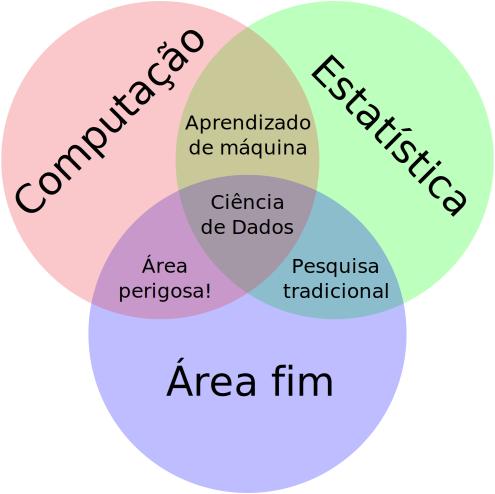
\includegraphics{ciencia-de-dados-diagrama-venn}
\caption{Diagrama de Venn mostrando as habilidades necessárias para um
cientista de dados}
\label{fig:ciencia-de-dados-venn}
\end{figure}

Com as técnicas da ciência de dados, podemos responder perguntas como ``Qual a
melhor rota para chegar até meu trabalho?'', ``Vai chover hoje?'', ``Quais são
minhas chances de desenvolver câncer nos próximos 10 anos?''. Neste trabalho,
estamos interessados nas técnicas de desenvolvimento de modelos preditivos que,
baseados nos dados e conhecimento que temos do assunto, determinam a
probabilidade de acontecimentos futuros.

\subsection{Modelos preditivos}

\citeonline{Geisser1993} define modelagem preditiva como sendo ``o processo
pelo qual um modelo é criado ou escolhido para tentar melhor prever a
probabilidade de um resultado''. Já \citeonline{Kuhn2013} definem como ``o
processo de desenvolvimento de uma ferramenta ou modelo matemático que gere uma
previsão precisa''.

Independente da definição usada, modelos preditivos fazem parte do dia-a-dia da
sociedade atual. O Google os utiliza para interpretar o que seus usuários estão
buscando; o Netflix usa para recomendar filmes; corretoras de valores usam para
definir que ações comprar ou vender; seguradoras usam para definir qual o risco
e, consequentemente, o preço do seguro de um carro, entre outros
\cite{Levy2010}.

Existem duas principais categorias de problemas que podem ser resolvidos por
modelos preditivos: regressão e classificação. A diferença entre eles está no
tipo de resposta que queremos prever, se é contínua ou categórica, que
influencia nos tipos de modelos que podem ser usados e na forma de avaliá-los.
Por exemplo, ao analisarmos modelos que preveem o preço de um imóvel a partir
da sua área, buscamos o que chegue mais próximo do valor real\footnote{Esta é
uma simplificação. Existem diversas outras características a serem analisados
ao escolher um modelo, como facilidade de interpretação, velocidade de
execução, entre outras. Aqui consideramos que a única diferença entre eles seja
o resultado previsto.}. Já ao avaliar modelos que classifiquem imagens dos
dígitos 0 a 9, só nos interessamos na classificação correta; dois modelos que
identifiquem a imagem do número 1 como sendo do número 3 e 8 estão igualmente
errados. O que classificou como 3 não está ``menos errado'' do que o que
classificou como 8 \cite{Kuhn2013,Zumel2014}. Neste trabalho, nosso foco é em
classificação.

\subsubsection{Modelos de classificação}

% TODO: Concluir

% % Treinamento de algoritmos
% % Regressão VS Classificação

% Random Forest
% % Árvores de decisão

% Validação cruzada

\section{Modelos espaciais de votação}



A ideia básica de modelos espaciais de votação é que o conjunto de alternativas
políticas de uma votação pode ser tratado como uma dimensão em um espaço
euclidiano, e cada parlamentar tem preferências de valores nessa dimensão. O
voto seria então definido pela escolha da alternativa mais próxima da sua
preferência.

Há diversos modelos para estimar esses valores, como o NOMINATE, W-NOMINATE,
DW-NOMINATE, que são paramétricos; o Optimal Classification, que é
não-paramétrico, e; modelos baseados em estatística Bayesiana, como o IDEAL.
Nosso foco neste trabalho é no W-NOMINATE.
\cite{Poole2000,Poole2005,Poole2014,Jackman2000,Clinton2004}

Considere um exemplo onde 5 parlamentares votam em
dois projetos de Lei: um propondo a redução da maioridade penal de
18 para 16 anos e outra
propondo o aumento do salário-mínimo de R\$ 1.000 para
R\$ 1.200. Suponha que cada um tem uma única preferência
(\emph{single-peakedness}), conhecido como seu ponto ideal, e vota sinceramente
de acordo com ela. Considere também que as preferências são simétricas. Isto é,
dado duas escolhas a uma mesma distância do ponto ideal de um parlamentar, ele
será indiferente a qualquer uma delas.

Graficamente, temos a figura \ref{fig:modelo-espacial-votacao}, onde os pontos
representam as preferências dos legisladores sobre cada votação, representados
como as dimensões nesse espaço euclidiano. As linhas são chamadas linhas de
corte. Elas passam pelo ponto médio entre as duas alternativas em votação: a de
votar sim e a de votar não. Em outras palavras, se as escolhas são entre uma
maioridade penal de 16 ou
18, a linha de corte passa em $\frac{16 + 18}{2}$,
ou seja, $17$. Ela divide os legisladores que irão votar não, que estão a
esquerda da linha, dos que irão votar sim, que estão a direita da mesma. Caso
esteja em cima da linha de corte, ele é indiferente as alternativas.

\begin{knitrout}
\definecolor{shadecolor}{rgb}{0.969, 0.969, 0.969}\color{fgcolor}\begin{figure}
\includegraphics[width=\maxwidth]{figure/tmp/modelo-espacial-votacao-1} \caption[Preferências de 5 deputados em 2 votações com suas respectivas linhas de corte]{Preferências de 5 deputados em 2 votações com suas respectivas linhas de corte}\label{fig:modelo-espacial-votacao}
\end{figure}


\end{knitrout}

Nesse exemplo estamos mostrando duas dimensões, mas o algoritmo é capaz de
estimar os pontos ideais em qualquer número de dimensões.

O comportamento dos parlamentares é assumido como sendo formado por dois
componentes: um determinístico e outro estocástico. Formalmente, definimos a
utilidade do legislador $i$ na consequência política do resultado ``sim'' da
votação $j$ como sendo:

\begin{equation}
  U_{ijy} = u_{ijy} + \epsilon_{ijy}
\end{equation}

onde $u_{ijy}$ é a parte determinística e $\epsilon_{ijy}$ é a parte
estocástica da função utilidade. Se não houver erro, o legislador vota sim se
$U_{ijy} > U_{ijn}$ e não se $U_{ijy} < U_{ijn}$. Caso $U_{ijy} = U_{ijn}$, ele
é indiferente para qualquer resultado.

\begin{description}
\item[$s$] o número de dimensões indexado por $k = 1, ..., s$;
\item[$p$] o número de parlamentares indexado por $i = 1, ..., p$;
\item[$q$] o número de votações indexado por $j = 1, ..., q$;
\item[$X_i$] o ponto ideal do parlamentar $i$ em um vetor de comprimento $s$;
\item[$Z_{jy}$ e $Z_{jn}$] a representação de cada votação em um vetor de comprimento
$s$, onde $y$ e $n$ são as consequências políticas dos resultados ``Sim'' e
``Não'', respectivamente.
\end{description}

A utilidade do parlamentar $i$ para a consequência $y$ em uma votação $j$ é:

\begin{equation}
  U_{ijy} = \beta \exp^{\left( - \frac{1}{2} \sum\limits_{k=1}^s w_k^2 d_{ijky}^2 \right)}
\end{equation}

Formalmente, sendo $O_{jy}$ e $O_{jn}$ os resultados correspondendo
respectivamente a um voto ``sim'' e um voto ``não'' na votação $j$ ($j = 1,
..., q$), definimos $Z_j$ como: 

\begin{equation}\label{eq:cutpoint}
  Z_j = \frac{O_{jy} + O_{jn}}{2}
\end{equation}

O $Z_j$ pode definir um ponto, linha, plano ou hiperplano, dependendo do número
de dimensões que estamos tratando. Ele é conhecido como ponto (ou linha, etc.)
de corte.

% Introdução

%% O que são de modelos de votação?

%% Por que os modelos espaciais de votação foram criados?

%% Por que não usar os votos diretamente?

% Desenvolvimento

% Conclusão

\subsection{Comparando pontos ideais ao longo do tempo}
\label{cap:fundamentacao:comparando-pontos-ideais-no-tempo}

O principal problema em comparar mudanças nos pontos ideais ao longo do tempo é
distinguir alterações causadas por mudanças na agenda legislativa das causadas
por mudanças no posicionamento dos parlamentares \cite{Bailey2007}. Em outras
palavras, se o ponto ideal de um deputado federal passa de 0.3 para -0.2 de um ano
para o outro, como descobrir se isso representa uma mudança real de ideologia ou
é somente reflexo da diferença na agenda legislativa dos dois períodos?

Segundo \citeonline{Shor2010}, todos os esforços para resolver esse problema
usam ``pontes'', que podem ser parlamentares cujo posicionamento assume-se ter
se mantido estável durante o período de interesse, ou; projetos de Lei que
foram votados em mais de um momento (nas duas casas legislativas em um sistema
bicameral, por exemplo). O primeiro é mais usado para comparar as mudanças nos
posicionamentos dos parlamentares, enquanto o segundo permite unir pessoas que
não votaram juntas em um mesmo mapa espacial\footnote{Por exemplo,
\citeonline{Shor2010} colocam todos os legisladores de 11 estados americanos e
do congresso federal em um período que varia entre 7 e 15 anos, dependendo do
estado, em um mesmo mapa espacial}. \citeonline{Poole2005} propõe duas formas
para estimar pontos ideais usando pontes.

Na primeira, batizada de \emph{pooled scaling} por \citeonline{Shor2010},
dividimos os votos dos parlamentares que queremos mensurar em dois
parlamentares ``virtuais'', um com os votos antes e outro com os votos depois
da data de interesse. Unimos esses parlamentares virtuais com os
parlamentares-ponte, que possuem um registro único, em uma tabela individual e
executamos o algoritmo de estimação dos pontos ideais. Ao final, teremos dois
pontos para cada parlamentar de interesse e um ponto para os pontes. Na
segunda, que \citeonline{Shor2010} chamam de \emph{linear mapping}, estimamos
os pontos ideias separadamente em cada período e os conectamos usando regressão
entre os conjuntos de pontos dos parlamentares-ponte. Ambas formas devem gerar
resultados similares, mas a segunda é computacionalmente mais simples, o que
pode ser essencial, dependendo da quantidade de parlamentares e votações votos
em estudo.

\citeonline{Poole2005} ainda descreve uma terceira forma, similar a
\emph{pooled scaling} descrita acima, que usa para testar se os senadores
norte-americanos mudam de comportamento nos últimos dois anos de seus mandatos,
antes de concorrer à reeleição. Neste caso, ele quer calcular a mudança de
comportamento de todos os legisladores em dois momentos numa mesma legislatura.
Se usássemos o \emph{pooled scaling} diretamente, precisaríamos escolher alguns
parlamentares como pontes que, por definição, não teriam mudado de
comportamento. Ao invés disso, ele segue o seguinte processo:

\begin{enumerate}
  \item Para cada parlamentar, faça:
    \begin{enumerate}
      \item Transforme-o em dois parlamentares ``virtuais'', um com o conjunto
de votos antes, e outro com os depois da data de interesse. Os outros
parlamentares não são modificados;
      \item Calcule os pontos ideias;
      \item Guarde os resultados dos dois parlamentares ``virtuais''. A
diferença entre suas posições representa a mudança de comportamento do
parlamentar.
    \end{enumerate}
  \item Calcule medidas de incerteza para as estimativas.
\end{enumerate}

Ao final, ele tem dois pontos para cada senador: um representando sua posição
nos primeiros 4, e o outro nos últimos 2 anos da legislatura. Note que, como as
matrizes de votações usadas para gerar os mapas espaciais são diferentes, eles
não são estritamente comparáveis. Apesar disso, \citeonline{Poole2005}
argumenta que como elas possuem o mesmo conjunto de votos, com a única
diferença de que um dos parlamentares foi dividido em dois, ele considera ser
seguro compará-las.

\section{Processo legislativo}

Como são criadas as Leis no Brasil? Essa seção pode ser gigantesca, então acho melhor focar no essencial e pontuar as características mais importantes para este trabalho, por exemplo o que são destaques, tipos de votação, tipos de votos, etc.

% ALEXANDRE: Acho que senado e câmara podem ser subseções desta seção.
% Essas subseções não precisam ser muito longas. Devem descrevas basicamente as competências e atribuições de cada casa.
%
% Acho que a justificativa da escolha da Câmara pode aparecer mais tarde, na seção do estudo de caso.  
% Assim a seção de fundamentação teórica fica sendo realmente apenas de fundamentação teórica, sem efeitos colaterais.

\subsection{Senado Federal}

Também chamada de Casa Alta, ela é composta por 81 senadores, 3 por cada Estado e Distrito Federal. Os senadores têm mandato de 8 anos e são eleitos pelo sistema majoritário\footnote{No sistema majoritário, o candidato mais votado é eleito. Nos anos em que são eleitos 2 senadores, os dois candidatos mais votados serão eleitos. Ele pressupõe um (ou dois) único candidatos por partido. É o mesmo sistema usado nas eleições para os chefes do Poder Executivo (presidente da República, governadores e prefeitos). Com exceção da eleição de senadores e prefeitos em cidades com menos de 200 mil habitantes, onde há um único turno, as eleições ocorrem em dois turnos. \cite{Carneiro2013}}. A renovação da casa é parcial, modificando $\frac{1}{3}$ e $\frac{2}{3}$ dos senadores alternadamente de 4 em 4 anos.

\subsection{Câmara dos Deputados}

Também chamada de Casa Baixa ou Casa do Povo, ela é composta por 513 deputados federais, cujo papel é representar o povo. Cada Estado ou Distrito Federal elege entre 8 e 70 deputados, proporcionalmente a sua população. Os deputados têm mandato de 4 anos, eleitos pelo sistema proporcional\footnote{No sistema proporcional os partidos registram vários candidatos para o mesmo cargo. Os votos recebidos por cada candidato são direcionados ao partido, que precisa atingir uma quantidade mínima de votos (chamado quociente eleitoral) para eleger ao menos um de seus candidatos. Nesse sistema, um candidato com menos votos pode se eleger, enquanto outro com mais votos não se elegeu, dependendo do partido de cada um deles. \cite{Carneiro2013,Bramatti2014}}. Diferente do Senado Federal, a renovação é total de 4 em 4 anos.

\section{Considerações Finais}
\chapter{Trabalhos Relacionados}\label{cap:trabalhos-relacionados}


\section{Análise do comportamento parlamentar}
\label{cap:trabalhos-relacionados:analise-comportamento}

No final da década de 80 e na de 90, diversos autores viam o sistema político
brasileiro como sendo altamente instável, com um Poder Executivo fraco,
obrigado a negociar com cada parlamentar individualmente para executar seu
plano de governo. Os parlamentares, preocupados somente com seus interesses
individuais e regionalistas, seriam indisciplinados, levando a
ingovernabilidade do país
\cite{Abranches1988,Lamounier1994,Mainwaring2001,Ames2003}.

Contrários a esse diagnóstico, \citeonline{Limongi1995} descreveram um cenário
muito diferente. O Executivo, por ter domínio sobre a agenda legislativa,
seria capaz de executar seu plano de governo negociando diretamente com os partidos
políticos, que seriam capazes de disciplinar seus parlamentares a votar
conforme suas indicações. Esse diagnóstico foi feito a partir da análise das
votações nominais na Câmara dos Deputados no período de 1989 a 1994. Nessa
análise, os autores calcularam a coesão interna de cada partido, usando o
\gls{IR}\footnote{O \glsfirst{IR} varia de 0 a 100, e é calculado subtraindo a
proporção dos votos minoritários dos majoritários. Ele é 0 quando o partido
está dividido, com metade votando sim e a outra metade votando não, e é 100
quando todos os parlamentares votam da mesma forma \cite{Rice1924}.}. Todos os
partidos apresentaram níveis de coesão relativamente altos, com o menos coeso,
o PDS, atingindo um \gls{IR} 75,70, e o mais coeso, o PT, com \gls{IR} 95,96.

Essas duas correntes foram tão distintas que \citeonline{Power2010} as dividiu
em ``pessimistas'' e ``otimistas''.

Figueiredo e Limongi continuaram analisando dados relacionados ao mesmo tempo,
focando em períodos e características distintos, que confirmaram o prognóstico.
A coletânea desses artigos gerou o livro ``Executivo e Legislativo na nova
ordem constitucional'' \cite{Figueiredo2001}.

Também usando métricas de coesão, \citeonline{Cheibub2009} concluem que o
Congresso brasileiro, ao contrário do previsto pelos pessimistas, é altamente
centralizado, com partidos e seus líderes capazes de disciplinar seus
parlamentares, evitando que estes ajam somente em busca de benefícios para si
mesmo e seus redutos eleitorais.

Além de cientistas políticos, jornalistas também têm usado técnicas semelhantes
para análise das votações. O Grupo Estado, dono do jornal Estado de São Paulo
(o Estadão), lançou em maio de 2012 a ferramenta Basômetro\footnote{Disponível
em \url{http://estadaodados.com/basometro/}.}, um site interativo que permite a
análise de como os parlamentares, individualmente e agregados por partido,
votaram, com dados a partir do primeiro governo de Lula em 2003. Além da
análise de cada votação, o Basômetro também calcula a taxa de
governismo\footnote{A taxa de governismo é calculada como o percentual de vezes
que os parlamentares votaram de acordo com a posição do governo.} dos partidos
e parlamentares, mostrando suas flutuações em cada mês \cite{Estadao2012}.

\citeonline{Dantas2014} organizaram uma coletânea de artigos escritos baseados
em análises feitas com o Basômetro gerando o livro ``Análise política \&
jornalismo de dados''.

Apesar de serem de interpretação e cálculo mais simples, métricas de coesão têm
alguns problemas. Em primeiro lugar, pela distância entre valores não ser
uniforme (por exemplo, a distância entre 40\% e 50\% não é necessariamente
igual a entre 50\% e 60\%), eles só ordenam os parlamentares. Há também um
baixo valor de números possíveis. Em $p$ votações, há $p + 1$ valores
possíveis. Por exemplo, em 3 votações, os parlamentares só podem assumir os
valores 0\%, 33\%, 66\% e 100\%. Por fim, o índice é calculado em relação a
algum ponto específico. Por exemplo, a taxa de governismo é calculada com base
no voto do governo, que normalmente é definido pela indicação ou voto do líder
do governo. Assim, ninguém pode ser mais governista do que o próprio líder, o
que é um pressuposto que precisa ser testado
\cite{Poole2005,McCarty2011,Izumi2013}. Para evitar essas limitações, diversos
autores usam modelos espaciais de votação (ver Seção
\ref{cap:fundamentacao:teoria-espacial-do-voto}).

No Brasil, o primeiro autor a usar esses modelos foi \citeonline{Leoni2002},
que analisou o posicionamento dos deputados federais entre 1991 e 1998 usando o
W-NOMINATE. \citeonline{Desposato2005b} usou o mesmo método para analisar o
efeito da mudança partidária no comportamento dos parlamentares.
\citeonline{Zucco2009} também usa o W-NOMINATE, dessa vez para entender os
fatores que influenciam o comportamento dos parlamentares, encontrando
que a ideologia não explica completamente seus comportamentos, e indicativos
que o presidente da República é um importante influenciador, especialmente
através da distribuição de cargos e recursos.

\citeonline{Freitas2012} analisam o significado da primeira dimensão, estimada
usando W-NOMINATE, na Câmara dos Deputados e no Senado Federal, concluindo que
ela está ligada ao conflito governo e oposição. \citeonline{Izumi2013} repete
essa análise no Senado Federal usando outro modelo, o \emph{Optimal
Classification}, chegando a mesma conclusão.

Além de técnicas específicas para gerar mapas espaciais de votação, alguns
autores usaram técnicas de redução de dimensionalidade mais gerais.
\citeonline{Trento2013} analisaram os dados da Câmara dos Deputados, Senado
Federal e Câmara Municipal de São Paulo usando \gls{ACP}\footnote{Do inglês,
\emph{Principal Component Analysis} (PCA).}, uma técnica estatística de redução
de dimensionalidade. Eles mapeiam um voto sim ou não nos valores 1 e 0, e
transformam o conjunto de votos dos parlamentares em pontos em um espaço
n-dimensional, onde cada dimensão representa uma votação. Como o número de
votações é alto, é difícil visualizar esses pontos. Assim, usam o \gls{ACP}
para colocar esses pontos em um espaço bidimensional, mantendo ao máximo suas
posições relativas. Dessa forma, quanto mais próximo estiverem dois
parlamentares (ou partidos), mais vezes eles votaram da mesma forma. O
resultado dessa pesquisa foi o Radar Parlamentar\footnote{Disponível em
\url{http://radarparlamentar.polignu.org}}, um site interativo no qual é
possível visualizar os diversos gráficos gerados, com as posições dos
legisladores e partidos a cada ano.

Usando uma técnica semelhante, a \gls{MCA}, \citeonline{Andrade2015} colocam os
deputados federais em um espaço bidimensional, mostrando aonde estaria o
presidente da Câmara dos Deputados, Eduardo Cunha (PMDB/RJ). Como ele não vota,
consideraram seu posicionamento como sendo igual ao do líder do PMDB na Câmara
no período. Eles também analisaram a similaridade dos deputados com o Eduardo
Cunha através do percentual de votos que deram iguais a ele, batizando essa
métrica de ``Cunhômetro''.

Apesar dessas técnicas estatísticas como a \gls{ACP} e \gls{MCA} serem
similares a técnicas como o W-NOMINATE, não encontramos trabalhos que validem
seu uso em dados de votação, o que pode dificultar a interpretação dos seus
resultados.

% FIXME: Citar o GovTrack.us e https://opengovdata.io/

\subsection{Análise da mudança de comportamento parlamentar}

O problema básico em comparar mudanças de comportamento ao longo do tempo é
distinguir alterações por causa de uma mudança de agenda das causadas por uma
real mudança das preferências dos parlamentares \cite{Bailey2007}. Em outras
palavras, se em um momento dois parlamentares votaram 90\% das vezes da mesma
forma, e em outro momento eles votaram 50\% das vezes, como definir se essa
mudança se deu porque eles mudaram seus posicionamentos, ou simplesmente porque
eles concordavam nas votações do primeiro momento, mas não nas do segundo?

Segundo \citeonline{Shor2010}, todos os esforços para resolver esse problema
usam ``pontes'', que são parlamentares que estiveram presentes em ambos
momentos e cujo posicionamento se assume ter se mantido estável. Podemos citar
como exemplos parlamentares que foram eleitos para mais de uma legislatura, ou
que mudaram de Casa (deputados federais que se tornam senadores). Projetos de
Lei também podem ser usados como ponte, caso eles tenham sido votados nas
instituições ou períodos de interesse.

No artigo, \citeonline{Shor2010} usam três tipos de pontes para colocar
parlamentares que serviram no nível estadual em ambas as casas\footnote{O
sistema legislativo norte-americano, ao contrário do brasileiro, é bicameral
tanto a nível federal quanto estadual (exceto o estado de Nebrasca, que só
possui um Senado estadual)}, federal em ambas as casas, e no tempo.
Parlamentares que serviram por múltiplas legislaturas tanto a nível estadual
quanto federal servem de ponte entre as legislaturas; legisladores que passam
da casa baixa para a casa alta (ou vice-versa) em nível estadual conectam as
respectivas casas, e; parlamentares que passam do nível estadual para atuar no
nível federal conectam o estado com o Congresso.

No Brasil, \citeonline{Leoni2002} analisa as posições dos deputados federais na
49\textordfeminine{} e 50\textordfeminine{} legislaturas não usando pontes, mas
sim a correlação de Pearson entre os pontos ideais. Ele encontrou correlações
altas, em torno de 0,80. Apesar disso, ele reconhece que uma limitação de seu
trabalho é que, nos períodos estudados, o governo sempre foi de direita, o que
poderia causar essa baixa mudança de pontos ideais. Além disso, como ele não
usou nenhuma técnica para diferenciar mudanças de comportamento de mudanças na
agenda legislativa (como as pontes), não é possível distinguir a razão desse
resultado com segurança.

\citeonline{Desposato2005b}, ao analisar o impacto das mudanças de partido no
comportamento dos parlamentares, usou o posicionamento dos legisladores que não
mudaram de partido como pontes. \citeonline{Izumi2013} faz uma pesquisa
semelhante, mas analisando a mudança de comportamento dos senadores que mudaram
de um partido dentro da coalizão governamental para um fora (ou vice-versa),
para entender o efeito da coalizão no comportamento dos parlamentares.

O Basômetro e o Radar Parlamentar não diferenciam mudanças de comportamento
reais das causadas por mudança da agenda legislativa
\cite{Estadao2012,Trento2013}.

Em geral, trabalhos que usam métricas de coesão interpretam as razões de
mudanças de comportamento usando métodos qualitativos, enquanto os que usam
pontos ideais usam métodos quantitativos.

\section{Aprendizagem de máquina na Ciência Política}
\label{ref:trabalhos-relacionados:data-science-polsci}

Os trabalhos encontrados que usam técnicas de aprendizagem de máquina no
âmbito da Ciência Política dividem-se em duas categorias: os que analisam
textos (como discursos) buscando entender seu conteúdo ou o posicionamento do
autor, e os que analisam projetos de lei tentando prever seus resultados.

Dos que fazem análise textual, \citeonline{Thomas2006} criaram um modelo que
classifica os discursos em debates sobre projetos de lei no congresso
estadunidense como sendo contrários ou favoráveis ao mesmo.
\citeonline{Quinn2006} criaram um modelo que extrai tópicos do texto de
discursos, validando-o nos dados do 105\textordmasculine{} ao
107\textordmasculine{} senado dos Estados Unidos. \citeonline{Yu2008}
determinam a filiação partidária dos parlamentares estadunidense a partir dos
seus discursos. \citeonline{Somasundaran2010} classificam autores de textos
publicados na Internet identificando seu posicionamento político a partir de
suas argumentações. Já \citeonline{Conover2011} fazem o mesmo com os usuários do
Twitter\footnote{Disponível em \url{http://twitter.com}.}, mas a partir da
frequência do uso de certas palavras.

Já na previsão do sucesso de projetos de lei, \citeonline{Gerrish2011} e
\citeonline{Goldblatt2012} desenvolveram modelos que acertaram mais de 90\% dos
resultados nos períodos estudados. \citeonline{Yano2012} fizeram uma análise
semelhante, mas focando em prever os projetos de lei que conseguirão passar das
discussões ocorridas em comissões e ser postos em votação.
\citeonline{Wang2012} preveem os resultados através de uma caminhada aleatória
em 3 grafos heterogêneos interconectados, sendo dois representando os
legisladores e um representando projetos de lei. Os legisladores estão
interligados caso tenham escrito ao menos um projeto juntos\footnote{Do inglês,
\emph{co-sponsorship}.}, e os projetos de lei interligados pela análise da
similaridade textual. Quando um legislador vota em um projeto de lei, um
vértice é criado entre seu nó e o do projeto. Ele criou dois grafos para os
legisladores como forma de criar dois tipos de ligação entre os legisladores e
os projetos de lei: uma para representar votos sim, e outra para votos não.

A empresa americana \citeonline{FiscalNote2015} desenvolve ferramentas para
monitoramento legislativo usando técnicas de ciência de dados. Uma delas, a
\emph{Prophecy}\footnote{Disponível em
\url{https://www.fiscalnote.com/prophecy}.} (do inglês, profecia), supostamente
prevê o resultado de projetos de lei com 94\% de acurácia. No Brasil, o
\gls{ELLO}, empresa ligada ao \gls{CEBRAP}, possui um produto similar.

\section{Considerações Finais}

Como visto na Seção \ref{cap:trabalhos-relacionados:analise-comportamento}, o
foco da literatura encontrada é na análise e interpretação do comportamento dos
parlamentares, seja usando métricas de coesão ou modelos espaciais de votação.
Na Seção \ref{ref:trabalhos-relacionados:data-science-polsci}, foram
apresentados trabalhos que aplicam técnicas de aprendizagem de máquina em temas
da ciência política, buscando descobrir o posicionamento de pessoas através dos
seus textos ou prever o resultado de votações.

Nesse levantamento bibliográfico, não foi encontrado nenhum autor que
desenvolva o objetivo deste trabalho: a detecção de mudanças de posicionamento
dos legisladores. O que parece ser mais próximo é a pesquisa feita pela empresa
americana \citeonline{FiscalNote2015} para o desenvolvimento do produto
\emph{Prophecy}, mas não foi possível analisar as semelhanças mais a fundo pois
o processo usado por eles não é divulgado.

Nesse sentido, considero a definição da metodologia para o desenvolvimento de
um modelo de detecção de mudança de posicionamento dos deputados federais
brasileiros como sendo o principal diferencial e contribuição deste trabalho.




\chapter{Miolo da sua dissertação}\label{cap:miolo}

Neste capítulo apresentaremos o processo de desenvolvimento, partindo da
definição dos objetivos e período de estudo, passando pela extração, limpeza e
transformação dos dados, que serão brevemente analisados para entendermos suas
características e, a partir delas, escolher possíveis modelos preditivos que
serão validados para chegar ao modelo final.

\section{Operacionalização dos dados}

% Universo de votações

O período de análise deste trabalho é composto pela 50\textordfeminine{},
51\textordfeminine{}, 52\textordfeminine{}, 53\textordfeminine{} e
54\textordfeminine{} legislaturas, compreendendo os 20 anos de 1995 até o
início de 2015, entre o primeiro mandato de Fernando Henrique Cardoso até o
final do primeiro mandato de Dilma Rousseff. As 48\textordfeminine{} e
49\textordfeminine{} legislaturas, iniciadas em 1987 e 1991 respectivamente,
foram excluídas pois segundo \citeonline{Freitas2008} neste período os
parlamentares ainda estão se acomodando as novas regras definidas pela
Constituição de 1998.

% Universo de parlamentares

% FIXME: Essa justificativa está fraca, e está misturada com a explicação de
% quais parlamentares são considerados.
A análise se restringe à Câmara dos Deputados pois o número de parlamentares é
maior (existem 513 deputados federais contra 81 senadores) e os dados estão
disponíveis mais facilmente no próprio site da Câmara. Considerei todos os
parlamentares que votaram ao menos uma vez na Câmara, por isso o número é maior
do que os 513 eleitos por legislatura.

A unidade de análise usada é o parlamentar. Ela foi escolhida pois, apesar de
grande parte da literatura apontar o papel fundamental dos partidos no
comportamento dos parlamentares \cite{Figueiredo2001,Santos2003}, trabalhar com
os dados desagregados nos permite perceber movimentações como quando um
parlamentar deixa um partido governista para entrar em um de oposição (ou
vice-versa).

% Universo de votos

Os deputados podem votar sim, não, nulo, branco, se abster ou obstruir
\cite{Carneiro2013}, mas o método W-NOMINATE usado neste trabalho só considera
votos sim ou não. Isso nos dá duas opções: mapear os outros tipos de votos como
sendo a favor ou contra (por exemplo, considerando abstenções como votos
contrários), ou ignorá-los. Para evitar possíveis problemas metodológicos ao
criar critérios desse tipo, desconsidero votos diferentes de sim ou não.

% Composição das coalizões

% FIXME: Esse texto tá confuso.
As coalizões são compostas pelos partidos que controlam ao menos um ministério.
Uma nova coalizão é formada em duas situações: i) na mudança de legislatura, e;
ii) na mudança do conjunto de partidos que controlam ministérios. Em outras
palavras, se um partido que não possuía nenhum ministério passa a ter ao menos
um, ou se um partido deixa de controlar algum ministério, uma nova coalizão é
formada. Esses critérios foram definidos por \citeonline{Figueiredo2007},
inspirada no trabalho de \citeonline{Muller2000}.


\section{Origem dos dados}



% Votações

% FIXME: Super confuso. Tentei usar uma linguagem menos técnica, mas falhei
% miseravelmente. Não ficou claro pra ninguém, nem os que conhecem a linguagem
% técnica nem os que não conhecem.
Os votos e votações foram extraídos diretamente do site da Câmara dos
Deputados. Apesar da Câmara disponibilizar uma \gls{API} para consulta desses
dados através de um programa, até a data de escrita deste trabalho esta
consulta só poderia ser feita individualmente, votação por votação. Para
desenvolver o modelo preditivo, precisamos ter acesso a todos os dados
localmente, então desenvolvi um programa\footnote{Disponível em:
\url{https://github.com/vitorbaptista/dados-abertos-camara.gov.br}} na
linguagem Python que, com o auxílio da biblioteca Scrapy, baixa todas as
votações \cite{Python276,Scrapy}. A tabela
\ref{table:estatisticas-legislaturas} mostra o número de deputados federais,
votos e votações por legislatura. Em média, temos 623,80
parlamentares e 332,04 votos em
477,80 votações a cada legislatura.
\nocite{CamaraDosDeputados2015}

\begin{table}
\centering
\begin{knitrout}
\definecolor{shadecolor}{rgb}{0.969, 0.969, 0.969}\color{fgcolor}
\begin{tabular}{r|r|r|r}
\hline
Legislatura & Deputados Federais & Votações & Votos\\
\hline
50 & 631 & 468 & 178603\\
\hline
51 & 624 & 419 & 155737\\
\hline
52 & 614 & 451 & 134461\\
\hline
53 & 606 & 619 & 192879\\
\hline
54 & 644 & 432 & 131552\\
\hline
\end{tabular}


\end{knitrout}
\caption{Número de deputados federais e votações por legislatura}
\label{table:estatisticas-legislaturas}
\end{table}

Durante o período de estudo, alguns partidos mudaram de nome ou se fundiram.
Para evitar que consideremos os parlamentares desses partidos como migrantes,
normalizamos os nomes dos partidos. No caso de mudanças de nomes usamos a sigla
do primeiro e do último nome. Por exemplo, o PFL se tornou o DEM, então usamos
a sigla PFL>DEM. Já no caso de fusões, usamos a sigla do maior partido na data
da fusão e do novo nome. Por exemplo, o PL se fundiu com o PRONA para formar o
PR, então temos PL>PR. Esta é a mesma normalização usada pelo \gls{CEBRAP} em
seu banco de dados legislativo \cite{Freitas2008}. A lista completa dos
partidos e seus nomes normalizados pode ser consultada no apêndice
\ref{apendice:lista-partidos}.

% Coalizão
A lista das coalizões foi obtida através do banco de dados
legislativos do \gls{CEBRAP}. Ela contém a data de início e fim e a composição
partidária de cada coalizão. Como trabalhamos com os parlamentares
individualmente, gerei outra lista que contém todas as entradas e saídas dos
deputados federais na coalizão dentro de uma mesma legislatura. Por exemplo,
apesar do deputado Arlindo Chinaglia (PT/SP) passar de oposição a governo
em 2003 com a eleição de Lula, não consideramos isso uma mudança pois ela
ocorreu entre legislaturas. Já a saída de Romário (PSB/RJ) da coalizão quando
seu partido se tornou oposição em 2013 é considerada, pois ocorreu dentro de
uma mesma legislatura.

\begin{knitrout}
\definecolor{shadecolor}{rgb}{0.969, 0.969, 0.969}\color{fgcolor}\begin{figure}
\includegraphics[width=\maxwidth]{figure/tmp/mudancas-mensais-de-coalizao-1} \caption[Número de deputados federais que mudaram de posicionamento, entrando ou saindo da coalizão entre a 50\textordfeminine{} e 54\textordfeminine{} legislaturas agrupados mês a mês]{Número de deputados federais que mudaram de posicionamento, entrando ou saindo da coalizão entre a 50\textordfeminine{} e 54\textordfeminine{} legislaturas agrupados mês a mês.}\label{fig:mudancas-mensais-de-coalizao}
\end{figure}


\end{knitrout}

A figura \ref{fig:mudancas-mensais-de-coalizao} mostra as
890 entradas e saídas da coalizão agrupadas
mensalmente que ocorreram durante o período de estudo. Há meses que concentram
as mudanças de posicionamento, possivelmente um reflexo da sazonalidade das
trocas de partido \cite{Araujo2000,Melo2004,Freitas2008}. A linha tracejada
marca a data da Resolução n\textordmasculine{} 22.610 do TSE, que em
25/10/2007 alterou o entendimento das
regras de fidelidade partidária, tornando-as mais restritas \cite{TSE2007}.
Percebe-se que essa mudança alterou a frequência de entradas e saídas na
coalizão, o que poderá influenciar na acurácia do nosso modelo.

\section{Estimando os pontos ideais}

O primeiro passo para se analisar uma mudança de comportamento é definir os
períodos de estudo. Por exemplo, para analisar o efeito da saída do PSB da
coalizão em outubro de 2013 no comportamento dos parlamentares, poderíamos
definir o período inicial como sendo do início da legislatura até a data da
saída do PSB, e o período final como sendo da saída do PSB até o final da
legislatura. Como o objetivo deste trabalho não é analisar um período
específico, mas criar um modelo que detecte mudanças na coalizão, não basta
definir um, mas sim um conjunto de períodos.

Ao definir esses períodos precisamos levar em consideração diversos fatores.
Períodos muito curtos, por exemplo uma semana antes e uma semana depois, podem
sofrer com a falta de votações suficientes ou serem demasiadamente
influenciados por votações anômalas. Já períodos muito longos, como 5 anos
antes e 5 anos depois, dificultam a interpretação dos resultados pois podem
conter diversas mudanças de comportamento. No mínimo, precisamos de um período
que contenha 20 votações cuja minoria responsável por ao menos 2,5\% dos
votos\footnote{Estes são os critérios padrão de inclusão de parlamentares e
votações do W-NOMINATE, que seguimos neste trabalho.}.

Baseado nisso, defini períodos de 12 meses dentro de uma mesma legislatura
divididos em duas partes de mesmo tamanho. Eles iniciam no primeiro dia de cada
mês, partindo de 01/Fev no primeiro ano da legislatura até o do penúltimo. Por
exemplo, na 54\textordfeminine{} legislatura, o primeiro período vai de
01/Fev/2011 até 01/Fev/2012 (dividido em 01/Ago/2011), e o último vai de
01/Fev/2014 até 01/Fev/2015. Existem 37 desses períodos por legislatura, 185
nas 5 legislaturas estudadas neste trabalho.

O próximo passo é estimar os pontos ideais de cada parlamentar em cada período.
Para isto, seguimos a metodologia de \citeonline{Poole2005} descrita na sessão
\ref{cap:fundamentacao:comparando-pontos-ideais-no-tempo}.
\citeauthor{Poole2005} sugere repetir as estimativas 101 vezes para calcular o
erro. Entretanto, o volume de dados que estamos trabalhando invibializa esse
número de repetições com os recursos computacionais que tenho
disponível\footnote{Por exemplo, usando um núcleo de um processador AMD
Opteron\texttrademark{} 6238 com 2,6 GHz o processamento dos pontos ideais de
um parlamentar em um período demora cerca de 1h45m. Considerando somente os 513
deputados eleitos por legislatura, o cálculo de todos os 37 períodos levaria
aproximadamente 18 meses. Todas as 5 legislaturas analisadas neste trabalho
levariam mais de 7 anos. O cálculo é facilmente paralelizável, diminuindo o
tempo necessário de acordo com o número de processadores, mas ainda assim não
foi possível usar 101 repetições neste trabalho.}. Por isto, escolhi fazer 10
repetições, o que diminuiu o tempo necessário em cerca de 90\%.

Até esse momento, temos uma tabela onde cada linha representa um parlamentar em
um período, e nas colunas temos seus pontos ideais e as respectivas estimativas
de erro. Em outras palavras, temos nossas variáveis independentes, agora
precisamos determinar a variável dependente: se o parlamentar entrou ou saiu da
coalizão ou se manteve como estava.

Para isso, precisamos definir qual o período antes de uma mudança de
posicionamento que o parlamentar começa a mudar de comportamento. Por exemplo,
considere que detectamos que um parlamentar que está fora da coalizão se
aproximou do governo entre o primeiro e o segundo semestre de 2011, mas só
entrou na coalizão em 2014. Consideramos que essa aproximação em 2011 foi
indício da sua entrada na coalizão em 2014? E se ela tivesse ocorrido em 2012?
Em outras palavras, precisamos definir qual o ``raio de influência'' de uma
entrada ou saída da coalizão.

Não há uma resposta única. Alguns parlamentares podem mudar de comportamento
anos antes de saírem (ou entrarem) na coalizão, enquanto outros podem não mudar
em momento algum. A hipótese fundamental deste trabalho é que eles mudam de
comportamento antes de mudar de posicionamento, caso contrário seria impossível
prever um a partir do outro. Formalmente, sendo $Data_{coaliz\tilde{a}o}$ a
data de entrada ou saída da coalizão, $Data_{mudan\textit{\c{c}}a}$ a data onde
o parlamentar mudou de comportamento, $Data_{inicial}$ e $Data_{final}$ as datas
iniciais e finais do período analisado, e $P = Data_{mudan\textit{\c{c}}a} -
Data_{coaliz\tilde{a}o} = Data_{final} - Data_{mudan\textit{\c{c}}a}$ a
distância da data inicial até a data de mudança, que é igual a da data de
mudança até a data final, nossa hipótese é que $Data_{mudan\textit{\c{c}}a} <
Data_{coaliz\tilde{a}o}$ e o período em que consideramos que uma mudança de
comportamento esteja relacionada a mudança de posicionamento compreende
$\left[Data_{mudan\textit{\c{c}}a} - \frac{P}{2}, Data_{mudan\textit{\c{c}}a} +
\frac{P}{2}\right]$. Precisamos definir $P$.

Para entender melhor, vejamos a figura \ref{fig:raio-de-influencia-coalizao}.
Nela são mostrados cinco períodos de análise de um parlamentar que mudou de
comportamento em $Data_{coaliz\tilde{a}o} - P$, representado pela mudança da
região branca para a região verde. No primeiro período,
\ref{fig:raio-de-influencia-coalizao1}, a $Data_{final}$ é igual ao momento de
mudança de comportamento. Neste período não consideramos que houve uma mudança
de posicionamento. Na figura \ref{fig:raio-de-influencia-coalizao2}, a mudança
de comportamento ocorre no ponto médio entre a $Data_{mudan\textit{\c{c}}a}$ e
a $Data_{final}$.  É a partir desse período que consideramos que o parlamentar
mudou de posicionamento. Na figura \ref{fig:raio-de-influencia-coalizao3}, a
$Data_{final} = Data_{coaliz\tilde{a}o}$, e a $Data_{mudan\textit{\c{c}}a}$
estimada se iguala a mudança real de comportamento em $Data_{coaliz\tilde{a}o}
- P$. Se nossa escolha de $P$ foi correta para este parlamentar, este deve o
período com a mudança de comportamento mais intensa. A figura
\ref{fig:raio-de-influencia-coalizao4} mostra o último período em que ainda
consideramos que houve uma mudança causada pela entrada ou saída da coalizão,
pois a partir dele o comportamento em $\left[Data_{inicial},
Data_{mudan\textit{\c{c}}a}\right]$ começa a se igualar ao em
$\left[Data_{mudan\textit{\c{c}}a}, Data_{final}\right]$. Na última figura, a
\ref{fig:raio-de-influencia-coalizao5}, o comportamento nos dois momentos do
período de estudo se igualam.

\begin{knitrout}
\definecolor{shadecolor}{rgb}{0.969, 0.969, 0.969}\color{fgcolor}\begin{figure}
\subfloat[A data final está no limite do raio de influência da coalizão.\label{fig:raio-de-influencia-coalizao1}]{\includegraphics[width=\maxwidth]{figure/tmp/raio-de-influencia-coalizao-1} }
\subfloat[O raio de influência da coalizão chega a metade do segundo período. A partir daqui começamos a considerar que houve uma mudança de posicionamento.\label{fig:raio-de-influencia-coalizao2}]{\includegraphics[width=\maxwidth]{figure/tmp/raio-de-influencia-coalizao-2} }
\subfloat[A data estimada de mudança se iguala a data real. Este é o período onde esperamos encontrar a maior mudança de comportamento.\label{fig:raio-de-influencia-coalizao3}]{\includegraphics[width=\maxwidth]{figure/tmp/raio-de-influencia-coalizao-3} }
\subfloat[A partir daqui, o comportamento começa a se igualar nos dois momentos de análise. Este é o último período em que consideramos que houve uma mudança de posicionamento.\label{fig:raio-de-influencia-coalizao4}]{\includegraphics[width=\maxwidth]{figure/tmp/raio-de-influencia-coalizao-4} }
\subfloat[O comportamento nos dois períodos se iguala. Esperamos que a diferença entre os pontos ideias dos dois momentos volte aos níveis da primeira figura.\label{fig:raio-de-influencia-coalizao5}]{\includegraphics[width=\maxwidth]{figure/tmp/raio-de-influencia-coalizao-5} }\caption[Diversos períodos de análise de um parlamentar que mudou de comportamento em ]{Diversos períodos de análise de um parlamentar que mudou de comportamento em $Data_{coalizao} - P$, representado pela mudança da região branca para a verde.}\label{fig:raio-de-influencia-coalizao}
\end{figure}


\end{knitrout}

Neste trabalho, defini $P$ como sendo 6 meses. Em outras palavras, os
parlamentares começariam a mudar de comportamento a partir de 6 meses antes da
definitiva entrada ou saída da coalizão. Ao final desse processo, teremos uma
tabela como a \ref{table:dataset-final}, onde as colunas representam:

\begin{description}
\item[antes] Ponto ideal no período anterior
\item[antes.sd] Estimativa de erro do ponto ideal do período anterior
\item[depois] Ponto ideal no período posterior
\item[depois.sd] Estimativa de erro do ponto ideal do período posterior
\item[mudou\_posicionamento] Indica se o parlamentar se manteve no seu
posicionamento, dentro ou fora da coalizão, ou mudou
\end{description}

\begin{table}
\centering
\begin{knitrout}
\definecolor{shadecolor}{rgb}{0.969, 0.969, 0.969}\color{fgcolor}
\begin{tabular}{r|r|r|r|l}
\hline
antes & antes.sd & depois & depois.sd & mudou\_posicionamento\\
\hline
0,55 & 0,02 & -0,40 & 0,03 & Sim\\
\hline
0,90 & 0,01 & 0,85 & 0,02 & Não\\
\hline
-0,30 & 0,01 & 0,40 & 0,01 & Sim\\
\hline
\end{tabular}


\end{knitrout}
\caption{Exemplo da tabela usada para treinar o algoritmo.}
\label{table:dataset-final}
\end{table}


\section{Preditores}

\subsection{Aspectos temporais}



Uma das principais características da migração partidária no Brasil é sua
distribuição no tempo \cite{Araujo2000,Melo2004,Freitas2008}. A partir de 1995,
ela se concentra nos meses de fevereiro do primeiro e terceiro ano da
legislatura e no período pré-eleitoral, que se encerra em outubro do ano
anterior as eleições \cite{Freitas2008,Lei9504/1997}. Nesta sessão,
analisaremos se esse padrão se repete também no subconjunto de deputados que
migram para partidos de posicionamento oposto, saindo ou entrando na coalizão.

Há duas formas de um parlamentar entrar ou sair da coalizão: quando seu partido
o faz, ou mudando de partido. Das 890 mudanças de
posicionamento no período de estudo,
50,79\% (452)
ocorreram por migrações e
49,21\% (438)
pelo partido ter entrado ou saído da coalizão. Consideramos a data de mudança
de posicionamento de formas diferentes em cada caso. Quando o partido como um
todo entra ou sai da coalizão, consideramos a data de mudança como a data de
início da coalizão. Já em uma mudança por migração, usamos a data da primeira
votação do parlamentar no novo partido\footnote{Idealmente, a data de mudança
por migração deveria ser a data em que o parlamentar se filiou ao novo partido.
Infelizmente, essa informação não está disponível através da \gls{API} da
Câmara para todas as legislaturas analisadas, então usei a data da primeira
votação no novo partido. Como 99\% dos parlamentares faltam no máximo 35
votações seguidas, as duas datas são próximas na maioria dos casos.}.

A figura \ref{fig:mudancas-de-posicionamento-geral} mostra o número de
deputados federais que mudaram de posicionamento entre a 50\textordfeminine{} e
54\textordfeminine{} legislaturas agregados por mês. Três meses, março, abril e
outubro, concentram
52,36\%
(466) das mudanças, o que pode
ser um indício que as mudanças de posicionamento seguem um padrão semelhante ao
das mudanças de partido.

\begin{knitrout}
\definecolor{shadecolor}{rgb}{0.969, 0.969, 0.969}\color{fgcolor}\begin{figure}
\includegraphics[width=\maxwidth]{figure/tmp/mudancas-de-posicionamento-geral-1} \caption[Número de deputados que mudaram de posicionamento entre a 50\textordfeminine{} e 54\textordfeminine{} legislaturas agregados por mês]{Número de deputados que mudaram de posicionamento entre a 50\textordfeminine{} e 54\textordfeminine{} legislaturas agregados por mês.}\label{fig:mudancas-de-posicionamento-geral}
\end{figure}


\end{knitrout}

Na figura \ref{fig:mudancas-de-posicionamento-por-migrantes}, separamos os
deputados que mudaram de posicionamento migrando de partido dos cujo próprio
partido entrou ou saiu da coalizão. O padrão temporal dos dois grupos é
visivelmente distinto. Os que migraram de partido mudaram de comportamento em
média 37,67 vezes por mês, com
29,87\%
(135) ocorrendo em outubro. Houve respectivamente
13,27\%
(60) e
11,28\%
(51) em março e fevereiro, os segundo e terceiro
meses com mais mudanças. Já os parlamentares cujos partidos entraram ou saíram
da coalizão mudaram de posicionamento em média
36,50 vezes por mês, com janeiro, março e
maio concentrando
46,8\%
(205) das mudanças.

\begin{knitrout}
\definecolor{shadecolor}{rgb}{0.969, 0.969, 0.969}\color{fgcolor}\begin{figure}
\includegraphics[width=\maxwidth]{figure/tmp/mudancas-de-posicionamento-por-migrantes-1} \caption[Número de deputados migrantes e não-migrantes que mudaram de posicionamento entre a 50\textordfeminine{} e 54\textordfeminine{} legislaturas agregados por mês]{Número de deputados migrantes e não-migrantes que mudaram de posicionamento entre a 50\textordfeminine{} e 54\textordfeminine{} legislaturas agregados por mês.}\label{fig:mudancas-de-posicionamento-por-migrantes}
\end{figure}


\end{knitrout}

Separamos os dados por legislatura na figura
\ref{fig:mudancas-de-posicionamento-por-migrantes-por-legislatura}. Os
migrantes continuam com um padrão parecido, com em média
32,06\%
das mudanças ocorrendo em outubro,
14,18\%
em março e
10,48\%
em fevereiro. Os não-migrantes não seguem um padrão único, mudando a cada
legislatura.

\begin{knitrout}
\definecolor{shadecolor}{rgb}{0.969, 0.969, 0.969}\color{fgcolor}\begin{figure}
\includegraphics[width=\maxwidth]{figure/tmp/mudancas-de-posicionamento-por-migrantes-por-legislatura-1} \caption[Número de deputados migrantes e não-migrantes que mudaram de posicionamento entre a 50\textordfeminine{} e 54\textordfeminine{} legislaturas agregados por mês e legislatura]{Número de deputados migrantes e não-migrantes que mudaram de posicionamento entre a 50\textordfeminine{} e 54\textordfeminine{} legislaturas agregados por mês e legislatura.}\label{fig:mudancas-de-posicionamento-por-migrantes-por-legislatura}
\end{figure}


\end{knitrout}

Na figura \ref{fig:mudancas-de-posicionamento-por-ano-da-legislatura},
agregarmos por ano da legislatura ao invés de mês. A grande maioria das
mudanças dos migrantes,
84,07\%
(380), estão concentradas no
primeiro e terceiro anos, seguindo o padrão temporal de migração descrito por
\citeonline{Freitas2008}. Já os não-migrantes continuam sem um padrão claro.
Como só consideramos mudanças dentro da mesma legislatura, só uma ocorreu no
primeiro ano, durante o segundo mandato de Lula, quando o PDT entrou na
coalizão em abril de 2007. As outras mudanças estão razoavelmente bem
espalhadas do segundo ao último ano das legislaturas, com a maioria ocorrendo
no segundo ano.

\begin{knitrout}
\definecolor{shadecolor}{rgb}{0.969, 0.969, 0.969}\color{fgcolor}\begin{figure}
\includegraphics[width=\maxwidth]{figure/tmp/mudancas-de-posicionamento-por-ano-da-legislatura-1} \caption[Número de deputados migrantes e não-migrantes que mudaram de posicionamento entre a 50\textordfeminine{} e 54\textordfeminine{} legislaturas agregados por ano da legislatura]{Número de deputados migrantes e não-migrantes que mudaram de posicionamento entre a 50\textordfeminine{} e 54\textordfeminine{} legislaturas agregados por ano da legislatura.}\label{fig:mudancas-de-posicionamento-por-ano-da-legislatura}
\end{figure}


\end{knitrout}

Separando os dados por mês e ano da legislatura, temos a figura
\ref{fig:mudancas-de-posicionamento-por-migrantes-por-ano-da-legislatura}. Nos
migrantes,
52,55\%
(103) das mudanças ocorrem
em outubro do terceiro ano, o limite para se filiar a um partido para concorrer
nas próximas eleições \cite{Lei9504/1997}. Os não-migrantes continuam sem um
padrão claro.

\begin{knitrout}
\definecolor{shadecolor}{rgb}{0.969, 0.969, 0.969}\color{fgcolor}\begin{figure}
\includegraphics[width=\maxwidth]{figure/tmp/mudancas-de-posicionamento-por-migrantes-por-ano-da-legislatura-1} \caption[Número de deputados que mudaram de posicionamento entre a 50\textordfeminine{} e 54\textordfeminine{} legislaturas agregados por mês e ano da legislatura]{Número de deputados que mudaram de posicionamento entre a 50\textordfeminine{} e 54\textordfeminine{} legislaturas agregados por mês e ano da legislatura.}\label{fig:mudancas-de-posicionamento-por-migrantes-por-ano-da-legislatura}
\end{figure}


\end{knitrout}

Em suma, os deputados que entram ou saem da coalizão migrando de partido
seguem um padrão temporal similar ao das migrações partidárias em geral
descrito por \citeonline{Freitas2008}, enquanto os que mudam de posicionamento
sem migrar de partido não têm um padrão claro.

\section{Desenvolvimento do modelo}



Ao retirar os parlamentares nos períodos em que não conseguimos estimar seu
ponto ideal por causa de nossos critérios, ficamos com 78.576
entradas na tabela. Dessas, 3,97\%
(3.117) são de deputados que mudaram
de posicionamento e 96,03\%
(75.459) que não. A tabela
\ref{table:changed-coalitions-per-legislature} mostra esses dados separadamente
para cada legislatura.

\begin{table}
\centering
\begin{knitrout}
\definecolor{shadecolor}{rgb}{0.969, 0.969, 0.969}\color{fgcolor}
\begin{tabular}{l|r|r|r|r|r}
\hline
  & 50 & 51 & 52 & 53 & 54\\
\hline
S & 0,04 & 0,04 & 0,07 & 0,02 & 0,03\\
\hline
N & 0,96 & 0,96 & 0,93 & 0,98 & 0,97\\
\hline
\end{tabular}


\end{knitrout}
\caption{Número de deputados que entraram ou saíram da coalizão por legislatura.}
\label{table:changed-coalitions-per-legislature}
\end{table}


\begin{knitrout}
\definecolor{shadecolor}{rgb}{0.969, 0.969, 0.969}\color{fgcolor}\begin{figure}
\includegraphics[width=\maxwidth]{figure/tmp/unnamed-chunk-9-1} \caption[Preferências de 5 deputados em 2 votações com suas respectivas linhas de corte]{Preferências de 5 deputados em 2 votações com suas respectivas linhas de corte}\label{fig:unnamed-chunk-9}
\end{figure}


\end{knitrout}

% Construindo os modelos

% Avaliando


% Objetivo
% % Quais dados precisamos?
% % Qual o período de estudo?
% % Devo definir o período de 1 ano dividido no meio aqui?

% ETL
% % CEBRAP + Câmara dos Deputados
% % Normalização dos partidos
% % Ignora abstenções
% % Considera todos que já votaram ao menos 20 vezes
% % Votações não-unânimes

% Data Analysis
% % Mostrar informações gerais sobre o conjunto de dados

% Modelagem
% % Vou usar só Random Forests? Por que? Se sim, por que não gbm?

% Validação
% % Talvez fosse bom treinar com as legislaturas 50~53 e testar com a 54, ou
% %   com partes dela, pra demonstrar como ele seria usado no dia-a-dia.

% Conclusão

\section{Considerações Finais}

Desenvolvi uma ferramenta que extrai dados de diversas fontes, os consolida, analisa e gera relatórios para os usuários. Cada parte pode ser modificada e expandida, e os dados (e algoritmos) podem ser usados por outras pessoas. Daqui falta validar que os algoritmos na parte de análise geram algo interessante.
\chapter{Conclusão}\label{cap:conclusao}

\section{Limitações}
\label{cap:conclusao:limitacoes}

\subsection{Definição dos períodos de análise}

Na sessão \ref{cap:miolo:estimando-pontos-ideais}, descrevi a metodologia usada
para analisar mudanças de comportamento baseado na de \citeonline{Poole2005}
descrita na sessão \ref{cap:fundamentacao:comparando-pontos-ideais-no-tempo}.
Nela, levantei três limitações deste trabalho: a definição da duração dos
períodos de análise, o número de repetições da estimativa dos pontos ideais para
calcular seu erro, e a definição do ``raio de influência'' de uma mudança de
posicionamento. Nesta sessão falarei sobre cada uma delas.

\subsubsection*{Duração dos períodos de análise}

Como o objetivo final deste trabalho não é análise, mas sim o desenvolvimento
de um modelo preditivo, precisei definir um conjunto de períodos de análise,
cujo tamanho foi definido arbitrariamente como um ano dividido em dois momentos
de seis meses. Uma forma possivelmente melhor seria analisar os dados para
encontrar o menor período que contenha o número de votações não-unânimes mínimo
definidos para o cálculo dos pontos ideais (neste trabalho, 20 votações com no
máximo 97,5\% votos para a maioria).

\subsubsection*{Raio de influência da mudança de posicionamento}

Uma vez definida a duração do período de análise, pode-se definir o raio de
influência buscando a maior mudança de comportamento entre os momentos dentro
do período. Por exemplo, digamos que o período definido seja de 12 meses
divididos em dois momentos de 6 meses cada. Poderíamos estimar os pontos ideais
nessa janela de tempo, buscando em que momento ocorre a maior alteração.


%%%%%%%%%%%%%%%%%%%%%%%%%%%%%%%%%%%%%%%%%%%%%%%%%%%%%%%%%%%%%%%%%%%%%%%%%%%%%%%%
%% BIbliografia
%% Coloque suas referencias no arquivo ref.bib

\bibliographystyle{abnt-alf} % estilo de bibliografia   plain,unsrt,alpha,abbrv.
\bibliography{ref} % arquivos com as entradas bib.

%Faz aparecer a referencia bibliografica no indice
\addcontentsline{toc}{section}{\numberline{}Referências Bibliográficas}

%%%%%%%%%%%%%%%%%%%%%%%%%%%%%%%%%%%%%%%%%%%%%%%%%%%%%%%%%%%%%%%%%%%%%%%%%%%%%%%%
%% Apendice
% Caso seja necessario algum apendice

\appendix
% TODO: Modificar o texto para não ficar igual a dissertação da Andréa e checar
% se faltam alguns partidos.

\chapter{Lista dos partidos}
\label{apendice:lista-partidos}

\begin{table}
\centering
\begin{tabular}{l l l l}
  Partido & Sigla agregada & Sigla atual & Nome atual \\
  \hline
  PFL>DEM & PFL>DEM & DEM & Democratas \\
  PCdoB & PCdoB & PCdoB & Partido Comunista do Brasil \\
  PDT & PDT & PDT & Partido Democrático Trabalhista \\
  PHS & PHS & PHS & Partido Humanista da Solidariedade \\
  PMDB & PMDB & PMDB & Partido do Movimento Democrático Brasileiro \\
  PMN & PMN & PMN & Partido da Mobilização Nacional \\
  PDS>PP\footnote{O PDS fundiu-se com o PDC em 1993, passando a chamar-se
Partido Progressista Reformador (PPR). Nova fusão com o PP em 21/09/1995 e nova
nomeclatura: Partido Progressista Brasileiro (PPB). Passa a denominar-se
Partido Progressista (PP) em 2003.} & PDS>PPR>PPB>PP & PP & Partido Progressista \\
  PCB>PPS\footnote{O Partido Comunista Brasileiro (PCB) mudou de nome para
Partido Popular Socialista (PPS) em 1991.} & PCB>PPS & PPS & Partido Popular Socialista \\
  PL>PR\footnote{Fusão do Partido Liberal (PL) com o PRONA em 2006, gestando o
Partido da República (PR).} & PL>PR & PR & Partido da República \\
  PMR>PRB\footnote{O Partido Municipalista Renovador (PMR) mudou a nomeclatura
para Partido Republicano Brasileiro (PRB) em 2006.} & PMR>PRB & PRB & Partido Republicano Brasileiro \\
  PRONA & PRONA & PRONA & Partido da Reedificação da Ordem Nacional \\
  PRTB & PRTB & PRTB & Partido Renovador Trabalhista Brasileiro \\
  PSB & PSB & PSB & Partido Socialista Brasileiro \\
  PSC & PSC & PSC & Partido Social Cristão \\
  PSD & PSD & PSD & Partido Social Democrático \\
  PSDB & PSDB & PSDB & Partido da Social Democracia Brasileira \\
  PSDC & PSDC & PSDC & Partido Social Democrata Cristão \\
  PSL & PSL & PSL & Partido Social Trabalhista \\
  PSOL & PSOL & PSOL & Partido Socialismo e Liberdade \\
  PST & PST & PST & Partido Social Trabalhista \\
  PSTU & PSTU & PSTU & Partido Socialista dos Trabalhadores Unificado \\
  PT & PT & PT & Partido dos Trabalhadores \\
  PTB & PTB & PTB & Partido Trabalhista Brasileiro \\
  PJ>PTC\footnote{O Partido da Juventude (PJ), fundado em 1985, mudou de nome
em 1989 para Partido da Reconstrução Nacional (PRN). Em 2001 passou a chamar-se
Partido Trabalhista Cristão (PTC)} & PJ>PRN>PTC & PTC & Partido Trabalhista Cristão \\
  PTN & PTN & PTN & Partido Trabalhista Nacional \\
  PV & PV & PV & Partido Verde \\
  SD & SD & SD & Solidariedade \\
\end{tabular}
\end{table}


\chapter{Versões dos softwares utilizados}

\begin{itemize}\raggedright
  \item R version 3.2.1 (2015-06-18), \verb|x86_64-pc-linux-gnu|
  \item Locale: \verb|LC_CTYPE=en_US.UTF-8|, \verb|LC_NUMERIC=C|, \verb|LC_TIME=pt_BR.UTF-8|, \verb|LC_COLLATE=en_US.UTF-8|, \verb|LC_MONETARY=pt_BR.UTF-8|, \verb|LC_MESSAGES=en_US.UTF-8|, \verb|LC_PAPER=pt_BR.UTF-8|, \verb|LC_NAME=C|, \verb|LC_ADDRESS=C|, \verb|LC_TELEPHONE=C|, \verb|LC_MEASUREMENT=pt_BR.UTF-8|, \verb|LC_IDENTIFICATION=C|
  \item Base packages: base, datasets, graphics, grDevices,
    methods, parallel, stats, utils
  \item Other packages: caret~6.0-47, doParallel~1.0.8,
    foreach~1.4.2, ggplot2~1.0.1, ggthemes~2.2.1, iterators~1.0.7,
    knitr~1.9, lattice~0.20-31, randomForest~4.6-10, scales~0.2.4,
    tikzDevice~0.8.1
  \item Loaded via a namespace (and not attached):
    BradleyTerry2~1.0-6, brglm~0.5-9, car~2.0-25,
    codetools~0.2-11, colorspace~1.2-4, digest~0.6.8,
    evaluate~0.5.5, filehash~2.2-2, formatR~1.2, grid~3.2.1,
    gtable~0.1.2, gtools~3.4.2, highr~0.5, labeling~0.3,
    lme4~1.1-7, MASS~7.3-42, Matrix~1.2-2, mgcv~1.8-6,
    minqa~1.2.4, munsell~0.4.2, nlme~3.1-121, nloptr~1.0.4,
    nnet~7.3-10, pbkrtest~0.4-2, plyr~1.8.2, proto~0.3-10,
    quantreg~5.11, Rcpp~0.11.4, reshape2~1.4.1, SparseM~1.6,
    splines~3.2.1, stringr~0.6.2, tools~3.2.1
\end{itemize}


%\chapter{Apêndice B}}\label{apendice-b}

%\chapter{Apêndice C}}\label{apendice-c}

%\chapter{Apêndice D}}\label{apendice-d}

%%%%%%%%%%%%%%%%%%%%%%%%%%%%%%%%%%%%%%%%%%%%%%%%%%%%%%%%%%%%%%%%%%%%%%%%%%%%%%%%

\end{document}
